\documentclass[12pt]{article}

\usepackage{amsmath}

\usepackage{graphicx}

\usepackage{hyperref}

\usepackage{graphicx}
\graphicspath{ {./images/} }


\usepackage[utf8]{inputenc}

\title{Operating System}
\author{Yuqiao Meng}
\date{2021–9–124}

\begin{document}

\maketitle

\newpage
\tableofcontents

\newpage

\section{Overview}

\subsection{What?}

What is an Operating System? What's its reponsibility?

\begin{itemize}
    \item A bunch of software and data residing somewhere in memory.
    \item The most privileged software in a computer. It  can do special things, like write to disk, talk over the network, control memory and CPU usage, etc
    \item Manages all system resources, including CPU, Memory, and I/O devices.
\end{itemize}

\subsection{Why?}
Why do we need an OS?
\begin{itemize}
    \item OS helps program to control hardwares.
    \item OS determines the way programs share resources.
    \item OS protects hardwares and programs from getting attacked.
    \item OS stores files persistently.
\end{itemize}
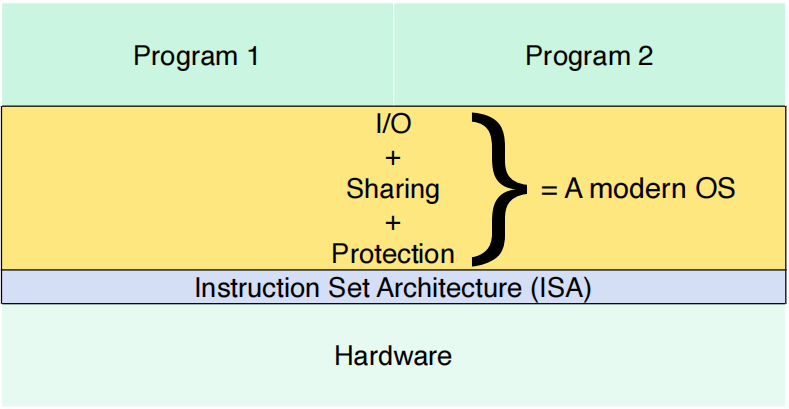
\includegraphics[width=1.0\textwidth]{WhyDoWeNeedOS.png}

\subsection{How}
\subsubsection{Virtulization}
\begin{itemize}
    \item Definition: OS takes a physical resource (such a sthe processor, or memory, or a disk) and transforms it into a more general, powerful, and easy-to-use virtual form of itself.
    \item Resource Virtulization \begin{itemize}
        \item Many(virtual)-to-one(physical): CPU Virtulization
        \item One-to-many: Disk Virtulization
        \item Many-to-many
    \end{itemize}
\end{itemize}
\subsubsection{How to invoke OS code?}
\begin{itemize}
    \item System calls: Function calls into the OS, that OS provides these calls to run programs, access memory and devices, and other related actions.
    \item Exceptions: CPU will raise an exception to the OS when the running program do something wrong
    \item Interrupts: Hardwares send interrupts to invoke OS
    \item Kernel Threads: Programs run in the kernel context, executing kernel level functions.
\end{itemize}
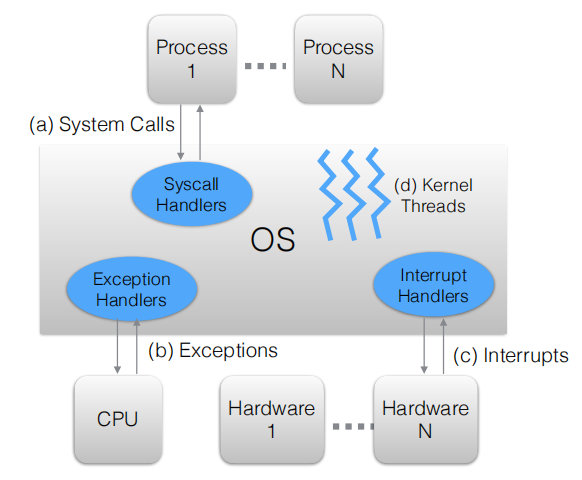
\includegraphics[width=0.8\textwidth]{FourWaysToInvokeOS.png}

\subsection{Interface}
\subsubsection{Explaination}
\begin{itemize}
    \item Instruction Set Architecture(ISA): the language CPU understand
    \item User ISA: ISA that any program can execute, it's accessible for all programs, doesn't need the service of operating system
    \item System ISA: ISA that only operating system is allowed to execute.
    \item Application Binary Interface(ABI): the combination of syscalls and User ISA(3, 7), it's the view of the world, seen by programs.
    \item Application Programmers' Interface(API): the combination of libraries and User ISA(2, 7), it's the tools programmer use to write codes.
\end{itemize}
\subsubsection{Interfaces in a Computer System}
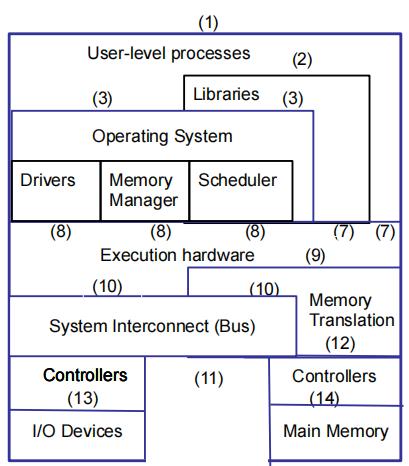
\includegraphics[width=0.6\textwidth]{InterfacesInComputerSystem.png}
\begin{itemize}
    \item User ISA: 7
    \item System ISA: 8
    \item Syscalls: 3
    \item Application Binary Interface: 3, 7
    \item Application Programmers' Interface: 2, 7
\end{itemize}

\subsection{History}
\begin{itemize}
    \item First Computer: Atanasoff–Berry computer, or ABC.
    \item First OS: GM-NAA I/O, produced in 1956 by General Motors' Research division for its IBM 704.
    \item First language: Plankalkül, developed by Konrad Zuse for the Z3 between 1943 and 1945.
    \item First programmer: Ada Lovelace
\end{itemize}

\end{document}